\documentclass[12pt]{article}

\input preamble

\title{Principles of Parallel Architecture\\
Fine Grain Synchronization}
\author{Xitong Liu \\
xliu@ece.udel.edu}

\begin{document}

\maketitle

\section{Dataflow}
Write a dataflow program that receives a token that contains an 
array with N numbers and produces these outputs:
\begin{enumerate}
\item The average of the numbers.
\item The standard deviation of the numbers.
\item The median of the numbers.
\end{enumerate}
\subsection{Average}
\begin{figure}[h!]
	\begin{center}
		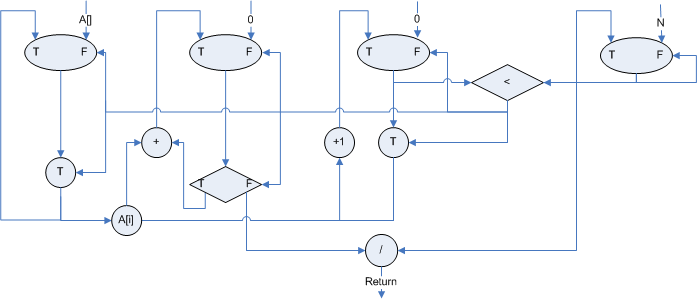
\includegraphics[width=1.1\textwidth, angle=0]{average.png}
		\caption{\label{fig:average}Dataflow Graph: Average of An Array}
	\end{center}
\end{figure}
\begin{equation}
\textsc{Average} = \frac{1}{N}\sum_{i=1}^{N}A[i]
\end{equation}

\subsection{Standard Deviation}
\begin{figure}[h!]
	\begin{center}
		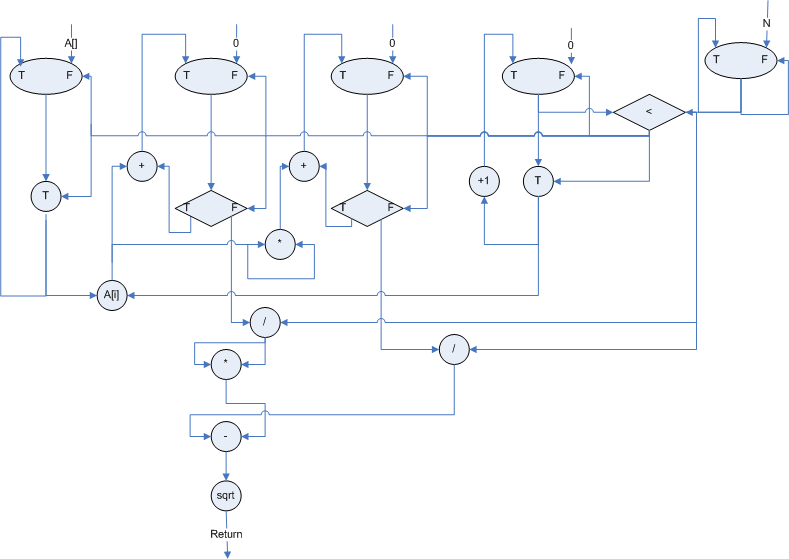
\includegraphics[width=1.1\textwidth, angle=0]{std-deviation.png}
		\caption{\label{fig:std-deviation}Dataflow Graph: Standard Deviation of An Array}
	\end{center}
\end{figure}
\begin{equation}
\textsc{Average} = \bar{A} =  \frac{1}{N}\sum_{i=1}^{N}A[i]
\end{equation}
\begin{align}
\textsc{StandardDeviation} &= \sqrt{\frac{1}{N}\sum_{i=1}^{N}(A[i]-\bar{A})^{2}} \nonumber\\
&= \sqrt{\frac{1}{N}(\sum_{i=1}^{N}A[i]^{2})-\bar{A}^{2}}
\end{align}

\subsection{Median}
\begin{figure}[h!]
	\begin{center}
		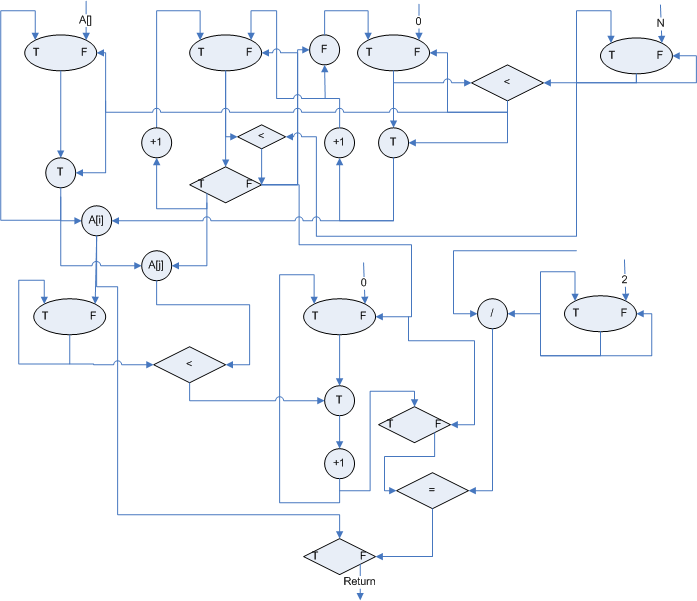
\includegraphics[width=1.1\textwidth, angle=0]{median.png}
		\caption{\label{fig:median}Dataflow Graph: Median of An Array}
	\end{center}
\end{figure}
The strategy of this program: from the beginning of the array, for each
element, count how many elements are less than the current one. If there 
are $\frac{N}{2}$ elements less than it, the current element is the median 
of the array.

\section{Questions}
\begin{enumerate}
\item
\begin{description}
\item[Q: ] What is the difference between loop execution in static and 
dynamic dataflow?
\item[A: ] For static dataflow, the token only contains value while for 
dynamic dataflow, the token contains both value and tag.
\end{description}

\item
\begin{description}
\item[Q: ] What are the advantages of architectures with single 
assignment rules?
\item[A: ] Single assignment rule can reduce the complexity of memory
management, make the program much simpler and easier to optimize.
\end{description}

\item
\begin{description}
\item[Q: ] Explain why it is difficult to achieve scalability of 
locks using traditional atomic operations and shared memory.
\item[A: ] To implement lock with shared memory, we have to 
synchronize updates to the shared memory structures. Since data
are shared and mutable, the synchronization overhead between the 
memory and cache lines becomes the bottleneck of scalability since
the complexity grows in $O(n)$ with the processors number.

\end{description}

\end{enumerate}

\end{document}

\begin{comment}
\begin{figure}[h!]
	\begin{center}
		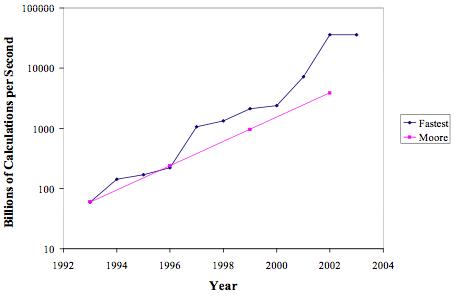
\includegraphics[width=0.7\textwidth, angle=0]{fatest.png}
		\caption{\label{fig:fatest}Fatest SuperComputer in the world}
	\end{center}
\end{figure}
\end{comment}
